\documentclass[12pt]{article}
\usepackage[paper=letterpaper,margin=2cm]{geometry}
\usepackage{amsmath}
\usepackage{amssymb}
\usepackage{amsfonts}
\usepackage{newtxtext, newtxmath}
\usepackage{enumitem}
\usepackage{titling}
\usepackage[colorlinks=true]{hyperref}
\usepackage{graphicx}
\usepackage{float}
\usepackage{listings}
\usepackage{xcolor}
\usepackage{color}
\usepackage{subfigure}
\definecolor{dkgreen}{rgb}{0,0.6,0}
\definecolor{gray}{rgb}{0.5,0.5,0.5}
\definecolor{mauve}{rgb}{0.58,0,0.82}
\lstset{ %
        language=Java,                
  basicstyle=\footnotesize,     
  numbers=left,               
  numberstyle=\tiny\color{gray},
  stepnumber=1,                                       
  numbersep=5pt,                 
  backgroundcolor=\color{white},  
  showspaces=false,             
  showstringspaces=false,         
  showtabs=false,                 
  frame=single,                   
  rulecolor=\color{black},       
  tabsize=4,                   
  captionpos=b,        
  breaklines=true,             
  breakatwhitespace=false,       
  title=\lstname,                                                  
  keywordstyle=\color{blue},          
  commentstyle=\color{dkgreen},    
  stringstyle=\color{mauve},       
  escapeinside={\%*}{*},        
  morekeywords={*,...}
} 

\setlength{\droptitle}{-6em}

% Enter the specific assignment number and topic of that assignment below, and replace "Your Name" with your actual name.
\title{Assignment 3: Comp 6771 Image Processing}
\author{Yunqi Xu 40130514}
\date{\today}



\begin{document}
% \maketitle

\begin{titlepage}
  \rule{\textwidth}{1pt}   % The top horizontal rule
    \vspace{0.2\textheight}  % Whitespace between top horizontal rule and title

    %------------------------------------------------------------
    %    Title
    %------------------------------------------------------------

    {\Huge COMP 6771 Image Processing: Assignment 2}

    \vspace{0.025\textheight}   % Whitespace between the title and short horizontal rule

    \rule{0.83\textwidth}{0.4pt}  % The short horizontal rule under title

    \vspace{0.1\textheight}  % Whitespace between the short horizontal rule and author

    %------------------------------------------------------------
    %    Author
    %------------------------------------------------------------

    {\Large Student name: \textsc{Yunqi Xu}}
    \vfill
    {\Large Student id: 40130514}
    \vfill  % Whitespace between author and date

    {\large \today}
    \vspace{0.1\textheight}  % Whitespace between date and bottom horizontal rule

    %------------------------------------------------------------
    %    Bottom rules
    %------------------------------------------------------------

    \rule{\textwidth}{1pt}  % The bottom horizontal rule
\end{titlepage}

\begin{enumerate}[leftmargin=\labelsep]
% \vspace*{40em}
\item Theoretical Question 1

    
    Based on the question, the mask is:
        \begin{equation}
            g(x, y) = \frac{1}{4}[f(x, y-1) + f(x, y+1) +f(x-1, y) +f(x+1, y)]  
            \label{q1_eq1}    
        \end{equation}
        Also, 
        \begin{equation}
            f(x - x_{0}, y - y_{0}) = F(u, v)e^{-j2 \pi (ux_{0}/M + vy_{0}/N)}
            \label{q1_eq2}
        \end{equation}

        Based on the Eq.~\ref{q1_eq2}, the Eq.~\ref{q1_eq1} can be calculated like:
        \begin{equation}
            \begin{aligned}
                f(x, y-1)
                &= f(x - 0, y -(1))\\
                &= F(u, v)e^{-j2\pi(u(0)/M + v(1)/N)}\\
                &= F(u, v)e^{-j2\pi v/N}
                \label{q1_eq3}
            \end{aligned}
        \end{equation}
        
        \begin{equation}
            \begin{aligned}
                f(x, y+1) 
                &= f(x-0, y-(-1))\\
                &= F(u, v)e^{-j2\pi (u(0)/M + v(-1)/N)}\\
                &= F(u, v)e^{j2\pi v/N}
            \label{q1_eq3}
            \end{aligned}
        \end{equation}

        \begin{equation}
            \begin{aligned}
                f(x-1, y) 
                &= f(x-(1), y-0)\\
                &= F(u, v)e^{-j2\pi(u(1)/M + v(0)/N)}\\
                &= F(u, v)e^{-j2\pi u/M}
            \label{q1_eq4}
            \end{aligned}
        \end{equation}

        \begin{equation}
            \begin{aligned}
                f(x+1, y) 
                &= f(x-(-1), y-0)\\
                &= F(u, v)e^{-j2\pi(u(-1)/M + v(0)/N)}\\
                &= F(u, v)e^{j2\pi u/M}
            \label{q1_eq5}
            \end{aligned}
        \end{equation}
        
        So, based on the Eq.~\ref{q1_eq2} ~\ref{q1_eq3} ~\ref{q1_eq4} ~\ref{q1_eq5}, 

        \begin{equation}
            G(u, v) = \frac{1}{4} F(u, v) [e^{-j2\pi v/N} + e^{j2\pi v/N} + e^{-j2\pi u/M} + e^{j2\pi u/M}]
        \end{equation}

        \begin{equation}
            H(u, v) = \frac{1}{4} [e^{-j2\pi v/N} + e^{j2\pi v/N} + e^{-j2\pi u/M} + e^{j2\pi u/M}]
        \end{equation}

        Based on the Euler's Formula, $\cos \theta = \frac{1}{2}(e^{i \theta} + e^{-i \theta})$,

        \begin{equation}
            \begin{aligned}
                H(u, v)
                &= \frac{1}{4}F(u, v)[2\cos(\frac{2 \pi v}{N} + 2\cos(\frac{2\pi u}{M}))]\\
                &= \frac{1}{2}F(u, v)[\cos(\frac{2 \pi v}{N} + \cos(\frac{2\pi u}{M}))]
            \end{aligned}
        \end{equation}

    \vspace*{7em}

\item Theoretical Question 2

\begin{enumerate}
    \item  If an equation is linear, which means that:
    \begin{equation}
        O(af_{1}(x, y) + bf_{2}(x, y)) = aO(f_{1}(x, y)) + bO(f_{2}(x, y))
        \label{q2_eq1}
    \end{equation}
    In Eq.~\ref{q2_eq1}, the $O()$ is an operator.
    So in this queation:
    \begin{equation}
        \begin{aligned}
        O(af_{1}(x, y) + bf_{2}(x, y))
        &= \int_{-\infty}^{\infty}\int_{-\infty}^{\infty}(af_1(x, y) + bf_2(x, y))\delta(x\cos\theta + y\sin\theta - \rho)dxdy\\
        &= a\int_{-\infty}^{\infty}\int_{-\infty}^{\infty}f_1(x, y)\delta(x\cos\theta + y\sin\theta - \rho)dxdy + \\
        & b\int_{-\infty}^{\infty}\int_{-\infty}^{\infty}f_2(x, y)\delta(x\cos\theta + y\sin\theta - \rho)dxdy\\
        &= aO(f_1(x, y)) + bO(f_2(x, y))
        % \label(q2_eq2)
        \end{aligned}
    \end{equation}
    So it is linear operator.

    \item Based on the priciple of Integral by substitution:
    \begin{equation}
     \begin{aligned}
        u = x - x_0\\
        v = y - y_0
        \end{aligned}
    \end{equation}

    \begin{equation}
        \begin{aligned}
            x = u + x_0\\
            y = v + y_0
        \end{aligned}
    \end{equation}

    \begin{equation}
        \begin{aligned}
            du = dx \\
            dv = dy
        \end{aligned}
    \end{equation}

    So, 
    \begin{equation}
        \begin{aligned}
                f(\rho, \theta)
                &= \int_{-\infty}^{\infty}\int_{-\infty}^{\infty}f(x - x_0, y - y_0) \delta(x\cos\theta + y\sin\theta - \rho)dxdy\\
                &= \int_{-\infty}^{\infty}\int_{-\infty}^{\infty}f(u, v)\delta[(u + x_0)\cos\theta + (v + y_0)\sin\theta - \rho)dudv\\
                &= \int_{-\infty}^{\infty}\int_{-\infty}^{\infty}f(u, v)\delta(u\cos\theta + x_0\cos\theta + v\sin\theta + y_0\sin\theta - \rho)dudv\\
                &= \int_{-\infty}^{\infty}\int_{-\infty}^{\infty}f(u, v)\delta(u\cos\theta + v\sin\theta - (\rho - x_0\cos\theta - y_0\sin\theta))dudv\\
                &= g(\rho - x_0\cos\theta - y_0\sin\theta, \theta)
        \end{aligned}
    \end{equation}    

\end{enumerate}

\item Programming Question 1 
\begin{enumerate}
\item The code is shown blow.
\begin{lstlisting}
    import numpy as np
    import cv2

    def imgread(path):
        return cv2.imread(path, 0)

    def generateHis(img, L):
        img_height, img_width = img.shape
        value_his = np.zeros(L)
        for y in range(img_height):
            for x in range(img_width):
                intensity = img[y,x]
                value_his[intensity] += 1
        value_prob = value_his * 1.0 / (img_height * img_width)
        return value_his, value_prob

    def Ostu(img, value_his, value_prob, L):
        img_height, img_width = img.shape
        final_var = 0
        var_list = []
        for k in range(1, L):
            p1 = np.sum(value_prob[:k])
            p2 = 1.0 - p1
            m1 = 0.0
            m2 = 0.0
            if p1 !=0 and p2 != 0:
                for i in range(k):
                    m1 += i * value_prob[i]
                m1 = m1/p1
                for j in range(k, L):
                    m2 += j * value_prob[j]
                m2 = m2/p2
                var = p1 * p2 * (m1- m2) **2
                var_list.append(var)

                if var > final_var:
                    final_var = var
            else:
                var_list.append(0)
        var_list = np.array(var_list)
        threshold_list = np.where(var_list == np.max(var_list))[0]
        threshold = np.average(threshold_list)
        return threshold

    def paddingReflect(img, kernel_size):
        # pre-processing:
        img_height, img_width= img.shape
        padded_img = np.zeros((img_height + kernel_size - 1, img_width + kernel_size - 1))
        padding_size = int((kernel_size - 1) / 2)
        padded_img[padding_size: padding_size + img_height, padding_size: padding_size + img_width] = img
        top_value = img[:padding_size, :]
        reversed_top_value = np.flip(top_value, axis = 0)
        padded_img[:padding_size, padding_size:padding_size+img_width] = reversed_top_value
        bottom_img_value = img[-padding_size:,:]
        reversed_bottom_value = np.flip(bottom_img_value, axis = 0)
        padded_img[-padding_size:,padding_size:padding_size+img_width] = reversed_bottom_value
        left_value = img[:, :padding_size]
        reversed_left_value = np.flip(left_value, axis = 1)
        padded_img[padding_size:padding_size+img_height, :padding_size] = reversed_left_value
        right_value = img[:, -padding_size:]
        reversed_right_value = np.flip(right_value, axis = 1)
        padded_img[padding_size:padding_size+img_height, -padding_size:] = reversed_right_value
        # 2. generate four corner
        lt_corner = img[:padding_size, :padding_size]
        reversed_lt_corner = np.flip(np.flip(lt_corner, axis=1), axis = 0)
        padded_img[:padding_size, :padding_size] = reversed_lt_corner
        rt_corner = img[:padding_size, -padding_size:]
        reversed_rt_corner = np.flip(np.flip(rt_corner, axis = 1), axis = 0)
        padded_img[:padding_size, -padding_size:] = reversed_rt_corner
        lb_corner = img[-padding_size:, :padding_size]
        reversed_lb_corner = np.flip(np.flip(lb_corner, axis = 1), axis = 0)
        padded_img[-padding_size:, :padding_size] = reversed_lb_corner
        rb_corner = img[-padding_size:, -padding_size:]
        reversed_rb_corner = np.flip(np.flip(rb_corner, axis = 1), axis = 0)
        padded_img[-padding_size:, -padding_size:] = reversed_rb_corner
        return padded_img

    def averagingFilter(input_image, filter_size):
        input_filter = np.zeros((filter_size, filter_size))
        image_height, image_width = input_image.shape[0],input_image.shape[1]
        output_image = np.zeros(input_image.shape)
        padding_size = int((filter_size - 1)/2)
        padded_image = paddingReflect(img=input_image, kernel_size=filter_size)

        for y in range(padding_size, image_height + padding_size):
            for x in range(padding_size, image_width + padding_size):
                sub_image = padded_image[y - padding_size: y + (padding_size + 1), x - padding_size: x + (padding_size +1)]
                output_image[y - padding_size, x - padding_size] = np.sum(sub_image)/(filter_size * filter_size)
        return output_image  

    img = imgread(path="tools_noisy.png")
    value_his, value_prob = generateHis(img=img, L = 256)
    th = Ostu(img=img, value_his=value_his, value_prob=value_prob, L=256)
    print(th)

    img[img<=th] = 0
    img[img>th] = 255
    cv2.imshow("test", img)
    cv2.imwrite("Figures/otsu_result.png", img)

    py_img = imgread(path="tools_noisy.png")
    retVal_b, b_img = cv2.threshold(py_img, 0, 255, cv2.THRESH_OTSU)
    print(retVal_b)
    cv2.imshow('test_2', b_img)
    cv2.imwrite("Figures/otsu_py.png", b_img)


    img = imgread(path = "tools_noisy.png")
    blur_img = np.uint8(averagingFilter(input_image=img, filter_size=7))
    blur_value_his, blur_value_prob = generateHis(img=blur_img, L = 256)
    blur_th = Ostu(img=blur_img, value_his=blur_value_his, value_prob=blur_value_prob, L=256)
    print(blur_th)
    blur_img[blur_img<=blur_th] = 0
    blur_img[blur_img>blur_th] = 255
    cv2.imshow("test blur", blur_img)
    cv2.imwrite("Figures/otsu_average.png", blur_img)

    py_img = imgread(path="tools_noisy.png")
    py_blur_img = cv2.blur(img, ksize=(7, 7), borderType=cv2.BORDER_REFLECT)
    retVal_b, blur_b_img = cv2.threshold(py_blur_img, 0, 255, cv2.THRESH_OTSU)
    print(retVal_b)
    cv2.imshow('test_blur python', blur_b_img)
    cv2.imwrite("Figures/otsu_py_average.png", blur_b_img)


    cv2.waitKey(0)
    cv2.destroyAllWindows()
\end{lstlisting}

\item The images are shown below:

    \begin{figure}[H]
        \centering
    
        \subfigure[Re-implement Otsu's algorithm]{
        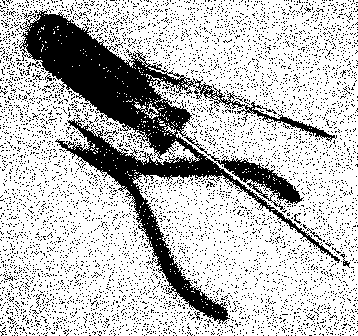
\includegraphics[width=7cm]{Figures/ostu_result.png}
        % \caption{fig1}
        }
        \quad
        \subfigure[Build-in python Otsu's algorithm]{
        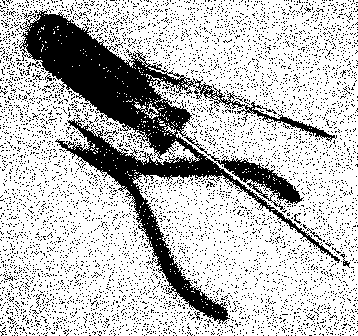
\includegraphics[width=7cm]{Figures/ostu_py.png}
        }
        \caption{Comparison of re-implement Otsu's algorithm and build-in Otsu's algorithm}
        \label{Q3_a}
    \end{figure}

The Fig.~\ref{Q3_a} presents the result between the re-implement Otsu's algorithm compared with the build-in python otsu's algorithm. 
And the result indicates that our re-implement can achieve the same output as the build-in python algorithm.


\item The Images are shown blow:
    \begin{figure}[H]
        \centering
        \subfigure[Re-implement Otsu's (with Averaging filter)]{
        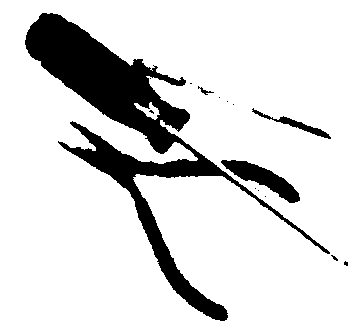
\includegraphics[width=7cm]{Figures/ostu_average.png}
        % \caption{fig1}
        }
        \quad
        \subfigure[Build-in python Otsu's (with Averaging fitler)]{
        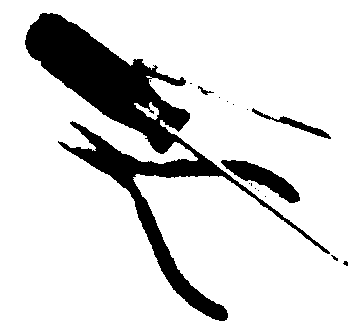
\includegraphics[width=7cm]{Figures/ostu_py_average.png}
        }
        \caption{Comparison of re-implement Otsu's and build-in Otsu's with averaging filter}
        \label{Q3_b}
    \end{figure}

The fig.~\ref{Q3_b} present the result between the re-implement Otsu's algorithm with averaging filter compared with the build-in python otsu's algorithm.
And the result indicates taht our re-implemnet can achieve the same output as the build-in python algorithm.
Compared with the Fig.~\ref{Q3_a} and Fig.~\ref{Q3_b}, the salt and pepper noises in Fig.~\ref{Q3_a} are removed after the averaing filter.

\end{enumerate}


\item Programming Q2
\begin{enumerate}
    \item The code is shown below
\begin{lstlisting}
    I = imread('lena.tif');

    % question a
    [c, s] = wavedec2(I, 3, 'haar');
    % level 1
    [H1, V1, D1] = detcoef2('all', c, s, 1);
    A1 = appcoef2(c, s, 'haar', 1);
    V1img = wcodemat(V1, 255, 'mat', 1);
    H1img = wcodemat(H1, 255, 'mat', 1);
    D1img = wcodemat(D1, 255, 'mat', 1);
    A1img = wcodemat(A1, 255, 'mat', 1);
    figure
    subplot(2, 2, 1);imagesc(A1img);colormap pink(255);title("(Haar) Approximation coef. of Level 1")
    subplot(2, 2, 2);imagesc(H1img);title("(Haar) Horizontal detail coef.level 1")
    subplot(2, 2, 3);imagesc(V1img);title("(Haar) Vertical detail coef. Level 1")
    subplot(2, 2, 4);imagesc(D1img);title("(Haar) Diagonal detail coef. Level 1")

    % level 2
    [H2, V2, D2] = detcoef2('all', c, s, 2);
    A2 = appcoef2(c, s, 'haar', 2);
    V2img = wcodemat(V2, 255, 'mat', 1);
    H2img = wcodemat(H2, 255, 'mat', 1);
    D2img = wcodemat(D2, 255, 'mat', 1);
    A2img = wcodemat(A2, 255, 'mat', 1);
    figure
    subplot(2, 2, 1); imagesc(A2img); colormap pink(255); title("(Haar) Approximation coef. of level 2")
    subplot(2, 2, 2); imagesc(H2img); title("(Haar) Horizontal detail coef. level 2")
    subplot(2, 2, 3); imagesc(V2img); title("(Haar) Vertical detail coef. level 2")
    subplot(2, 2, 4); imagesc(D2img); title("(Haar) Diagonal detail coef. level 2")

    % level 3
    [H3, V3, D3] = detcoef2('all', c, s, 3);
    A3 = appcoef2(c, s, 'haar', 3);
    V3img = wcodemat(V3, 255, 'mat', 1);
    H3img = wcodemat(H3, 255, 'mat', 1);
    D3img = wcodemat(D3, 255, 'mat', 1);
    A3img = wcodemat(A3, 255, 'mat', 1);
    figure
    subplot(2, 2, 1); imagesc(A3img); colormap pink(255); title("(Haar) Approximation coef. of level 3")
    subplot(2, 2, 2); imagesc(H3img); title("(Haar) Horizontal detail coef. level 3")
    subplot(2, 2, 3); imagesc(V3img); title("(Haar) Vertical detail coef. level 3")
    subplot(2, 2, 4); imagesc(D3img); title("(Haar) Diagonal detail coef. level 3")
\end{lstlisting}

    \begin{figure}[H]
        \centering
        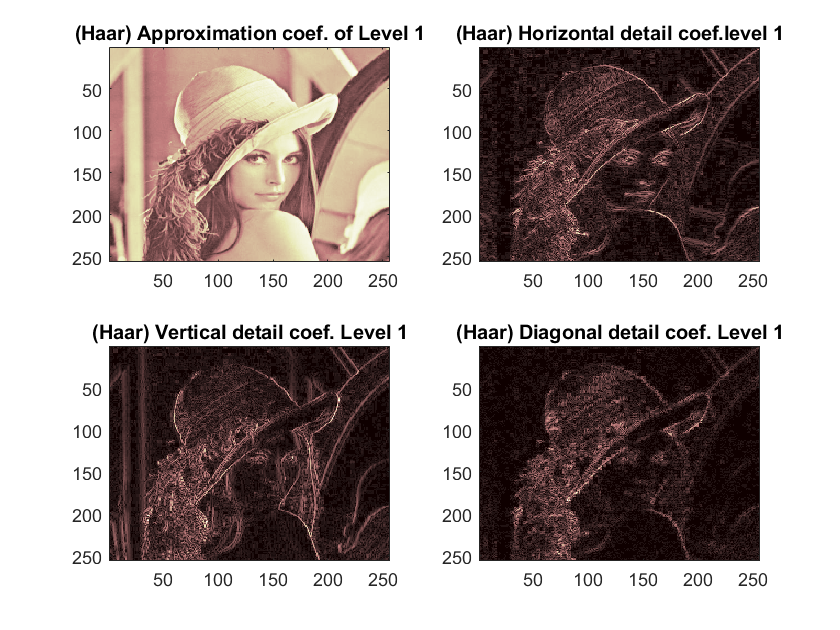
\includegraphics[width=0.5\textwidth,height=0.5\textwidth]{Figures/Haar1.png}
        \caption{Haar level 1}
        \label{Q4_a_level1}
    \end{figure}
    \begin{figure}[H]
        \centering
        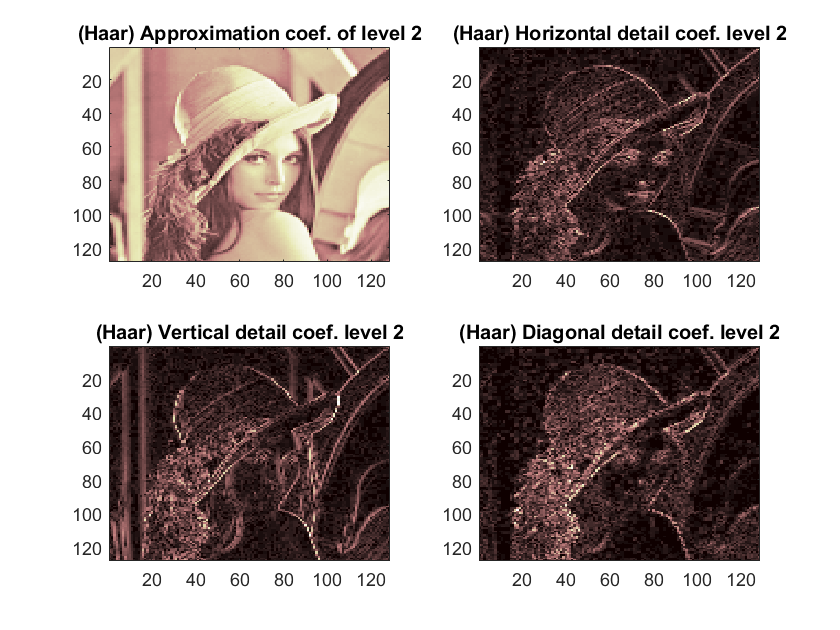
\includegraphics[width=0.5\textwidth,height=0.5\textwidth]{Figures/Haar2.png}
        \caption{Haar level 2}
        \label{Q4_a_level2}
    \end{figure}

    \begin{figure}[H]
        \centering
        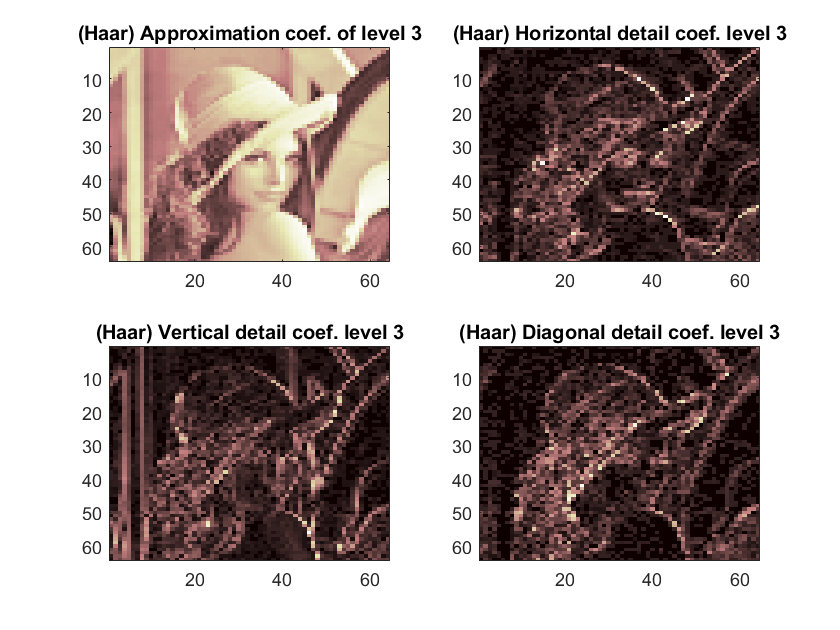
\includegraphics[width=0.5\textwidth,height=0.5\textwidth]{Figures/Haar3.png}
        \caption{Haar level 3}
        \label{Q4_a_level3}
    \end{figure}
    
    Fig.~\ref{Q4_a_level1}, ~\ref{Q4_a_level2}, ~\ref{Q4_a_level3} shown the result of the output $Wavedec2()$ using Haar wavelet. 


    \item  The code is showing below:
\begin{lstlisting}
    I = imread('lena.tif');

    % question b
    [c, s] = wavedec2(I, 3, 'db4');
    % level 1
    [H1, V1, D1] = detcoef2('all', c, s, 1);
    A1 = appcoef2(c, s, 'db4', 1);
    V1img = wcodemat(V1, 255, 'mat', 1);
    H1img = wcodemat(H1, 255, 'mat', 1);
    D1img = wcodemat(D1, 255, 'mat', 1);
    A1img = wcodemat(A1, 255, 'mat', 1);
    figure
    subplot(2, 2, 1);imagesc(A1img);colormap pink(255);title("(DB4)Approximation coef. of Level 1")
    subplot(2, 2, 2);imagesc(H1img);title("(DB4) Horizontal detail coef. of level 1")
    subplot(2, 2, 3);imagesc(V1img);title("(DB4) Vertical detail coef. of Level 1")
    subplot(2, 2, 4);imagesc(D1img);title("(DB4) Diagonal detail coef. of Level 1")

    % level 2
    [H2, V2, D2] = detcoef2('all', c, s, 2);
    A2 = appcoef2(c, s, 'db4', 2);
    V2img = wcodemat(V2, 255, 'mat', 1);
    H2img = wcodemat(H2, 255, 'mat', 1);
    D2img = wcodemat(D2, 255, 'mat', 1);
    A2img = wcodemat(A2, 255, 'mat', 1);
    figure
    subplot(2, 2, 1); imagesc(A2img); colormap pink(255); title("(DB4) Approximation coef. of level 2")
    subplot(2, 2, 2); imagesc(H2img); title("(DB4) Horizontal detail coef. of level 2")
    subplot(2, 2, 3); imagesc(V2img); title("(DB4) Vertical detail coef. of level 2")
    subplot(2, 2, 4); imagesc(D2img); title("(DB4) Diagonal detail coef. of level 2")

    % level 3
    [H3, V3, D3] = detcoef2('all', c, s, 3);
    A3 = appcoef2(c, s, 'db4', 3);
    V3img = wcodemat(V3, 255, 'mat', 1);
    H3img = wcodemat(H3, 255, 'mat', 1);
    D3img = wcodemat(D3, 255, 'mat', 1);
    A3img = wcodemat(A3, 255, 'mat', 1);
    figure
    subplot(2, 2, 1); imagesc(A3img); colormap pink(255); title("(DB4) Approximation coef. of level 3")
    subplot(2, 2, 2); imagesc(H3img); title("(DB4) Horizontal detail coef. of level 3")
    subplot(2, 2, 3); imagesc(V3img); title("(DB4) Vertical detail coef. of level 3")
    subplot(2, 2, 4); imagesc(D3img); title("(DB4) Diagonal detail coef. of level 3")   
\end{lstlisting}
    
    \begin{figure}[H]
        \centering
        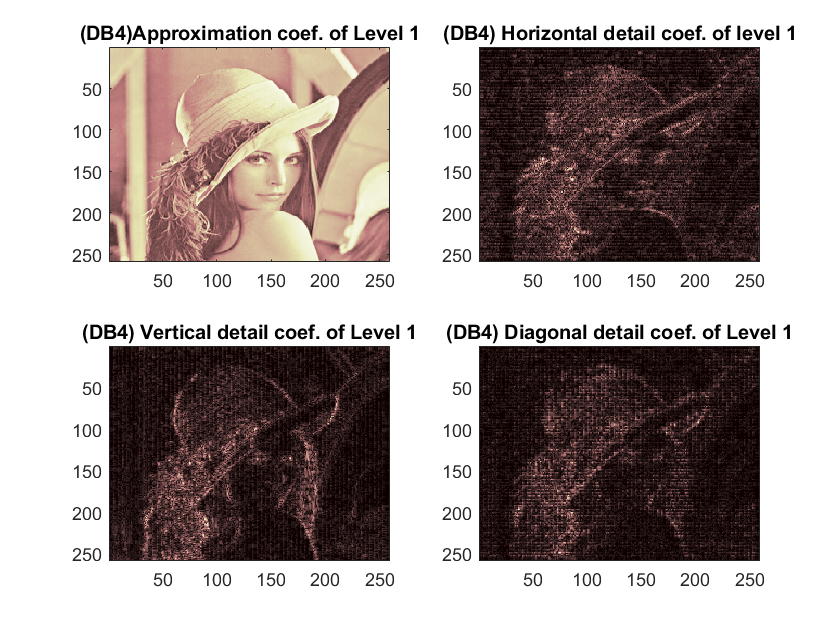
\includegraphics[width=0.7\textwidth,height=0.7\textwidth]{Figures/DB_1.png}
        \caption{Daubechies-4 level 1}
        \label{Q4_b_level1}
    \end{figure}
    \begin{figure}[H]
        \centering
        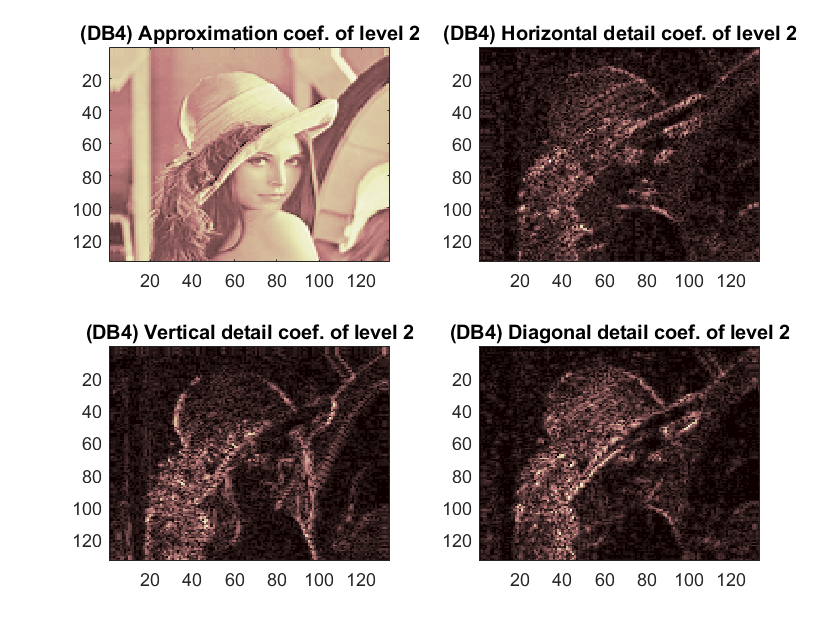
\includegraphics[width=0.7\textwidth,height=0.7\textwidth]{Figures/DB_2.png}
        \caption{Daubechies-4 level 2}
        \label{Q4_b_level2}
    \end{figure}

    \begin{figure}[H]
        \centering
        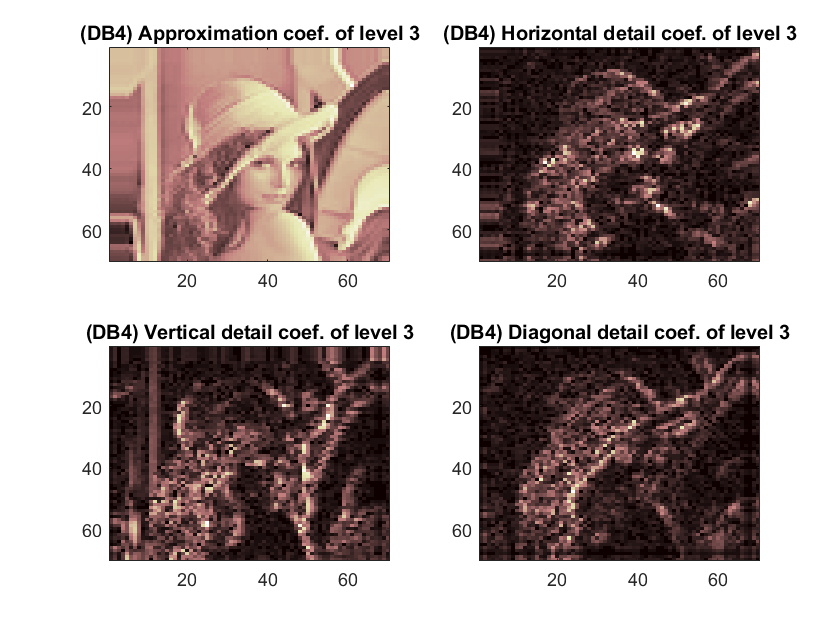
\includegraphics[width=0.7\textwidth,height=0.7\textwidth]{Figures/DB_3.png}
        \caption{Daubechies-4 level 3}
        \label{Q4_b_level3}
    \end{figure}
    
    Fig.~\ref{Q4_b_level1}, ~\ref{Q4_b_level2}, ~\ref{Q4_b_level3} present the result of the Daubechies4 wavelet.

    \item The figure present the comparison between the level 3 approximation image of Haar and the lavel 3 approximation image of Daubechies4.
    The result indicates that the Daubechies4 has a more smooth result compared with the result of Haar.
    
    \begin{figure}[H]
        \centering
        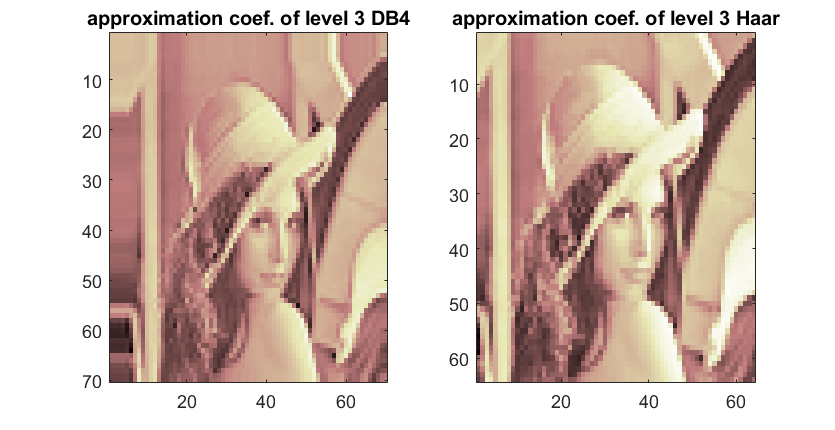
\includegraphics[width=0.7\textwidth, height=0.5\textwidth]{Figures/compare.png}
        \caption{Comparison between Haar and Daubechies-4 in level 3}
        \label{Q4_c_compare}
    \end{figure}

\end{enumerate}

\end{enumerate}

\end{document}
